\documentclass[titlepage, a4paper]{article}
\usepackage[swedish]{babel}
\usepackage[utf8]{inputenc}
\usepackage{color}
\usepackage{graphicx}
\usepackage{etoolbox}
\usepackage{stringenc}
\usepackage{pdfescape}

% Sidformat
\usepackage{a4wide}

% Fixa Appendix-titlar
\usepackage[titletoc,title]{appendix}

% Bättre tabeller
\usepackage{tabularx}

% Bättre bildtexter
\usepackage[margin=10pt,font=small,labelfont=bf,labelsep=endash]{caption}

% Enkelt kommando som låter mig attgöra-markera text
\newcommand{\todo}[1] {\textbf{\textcolor{red}{#1}}}

% Nytt \paragraph låter oss ha onumrerade bitar
\makeatletter
\renewcommand\paragraph{\@startsection{paragraph}{4}{\z@}%
{-3.25ex\@plus -1ex \@minus -.2ex}%
{1.5ex \@plus .2ex}%
{\normalfont\normalsize\bfseries}}
\makeatother

\providecommand{\LIPSlogga}{../mall/logga1.png}
\providecommand{\LIPSdatum}{\today}

%% Headers och Footers
\usepackage{fancyhdr}
\pagestyle{fancy}
\lhead{\includegraphics[scale=0.4]{\LIPSlogga}}
\rhead{\ifdef{\LIPSutfardare}{Utfärdat av \LIPSutfardare \\\LIPSdatum}\LIPSdatum}
\lfoot{\LIPSkursnamn \\ \LIPSdokumenttyp}
\cfoot{\thepage}
\rfoot{\LIPSprojektgrupp \\ \LIPSprojektnamn}

%% Titelsida
\newcommand{\LIPSTitelsida}{%
{\ }\vspace{45mm}
\begin{center}
  \textbf{\Huge \LIPSdokument}
\end{center}
\begin{center}
  {\Large Grupp: \LIPSgrupp}
\end{center}
\begin{center}
  {\Large Redaktör: \LIPSredaktor}
\end{center}
\begin{center}
  {\Large \textbf{Version \LIPSversion}}
\end{center}
\vfill
\begin{center}
  {\large Status}\\[1.5ex]
  \begin{tabular}{|*{3}{p{40mm}|}}
    \hline
    Granskad & \LIPSgranskare & \LIPSgranskatdatum \\
    \hline
    Godkänd & \LIPSgodkannare & \LIPSgodkantdatum \\
    \hline
  \end{tabular}
\end{center}
\newpage
}

% Projektidentitet
\newenvironment{LIPSprojektidentitet}{%
{\ }\vspace{45mm}
\begin{center}
  {\Large PROJEKTIDENTITET}\\[0.5ex]
  {\small
  \LIPSartaltermin, \LIPSprojektgrupp\\
  Linköpings Tekniska Högskola, IDA
  }
\end{center}
\begin{center}
  {\normalsize Gruppdeltagare}\\
  \begin{tabular}{|l|l|p{25mm}|l|}
    \hline
    \textbf{Namn} & \textbf{Ansvar} & \textbf{Telefon} & \textbf{E-post} \\
    \hline
}%
{%
    \hline
  \end{tabular}
\end{center}
\begin{center}
  {\small
    \ifdef{\LIPSgruppadress}{\textbf{E-postlista för hela gruppen}: \LIPSgruppadress\\}{}
    \ifdef{\LIPSgrupphemsida}{\textbf{Hemsida}: \LIPSgrupphemsida\\[1ex]}{}
    \ifdef{\LIPSkund}{\textbf{Kund}: \LIPSkund\\}{}
    \ifdef{\LIPSkundkontakt}{\textbf{Kontaktperson hos kund}: \LIPSkundkontakt\\}{}
    \ifdef{\LIPSkursansvarig}{\textbf{Kursansvarig}: \LIPSkursansvarig\\}{}
    \ifdef{\LIPShandledare}{\textbf{Handledare}: \LIPShandledare\\}{}
  }
\end{center}
\newpage
}
\newcommand{\LIPSgruppmedlem}[4]{\hline {#1} & {#2} & {#3} & {#4} \\}

%% Dokumenthistorik
\newenvironment{LIPSdokumenthistorik}{%
\begin{center}
  Dokumenthistorik\\[1ex]
  %\begin{small}
    \begin{tabular}{|l|l|p{60mm}|l|l|}
      \hline
      \textbf{Version} & \textbf{Datum} & \textbf{Utförda förändringar} & \textbf{Utförda av} & \textbf{Granskad} \\
      }%
    {%
			\hline
    \end{tabular}
  %\end{small}
\end{center}
}

\newcommand{\LIPSversionsinfo}[5]{\hline {#1} & {#2} & {#3} & {#4} & {#5} \\}

% Kravlistor
\newenvironment{LIPSkravlista}{
	\center
		\tabularx{\textwidth}{| p{1.2cm} | p{1.9cm} | X | c |}
			\hline
			\textbf{Krav} & \textbf{Förändring} & \textbf{Beskrivning} & \textbf{Prioritet} \\\hline
}
{
		\endtabularx
	\endcenter
}

\newcounter{LIPSkravnummer}
\addtocounter{LIPSkravnummer}{1}
\newcommand{\LIPSkrav}[4][Krav \arabic{LIPSkravnummer}]{{#1} & {#2} & {#3} & {#4} \stepcounter{LIPSkravnummer}\\\hline}


% Leveranskravlistor
\newenvironment{LIPSleveranskravlista}{
	\center
		\tabularx{\textwidth}{| p{1.2cm} | p{1.9cm} | X | X |}
			\hline
			\textbf{Krav} & \textbf{Förändring} & \textbf{Beskrivning} & \textbf{Deadline}\\\hline
}
{
		\endtabularx
	\endcenter
}

\newcounter{LIPSleveranskravnummer}
\addtocounter{LIPSleveranskravnummer}{1}
\newcommand{\LIPSleveranskrav}[4][Krav \arabic{LIPSkravnummer}]{{#1} & {#2} & {#3} & {#4} \stepcounter{LIPSkravnummer}\\\hline}


% Milstolps-lista
\newenvironment{LIPSmilstolpar}{
	\center
		\tabularx{\textwidth}{| p{1.2cm} | X | l |}
			\hline
			\textbf{Nr} & \textbf{Beskrivning} & \textbf{Datum} \\\hline
}
{
		\endtabularx
	\endcenter
}

\newcounter{LIPSstolpnummer}
\addtocounter{LIPSstolpnummer}{1}
%\newcommand{\LIPSmilstolpe}[3][Krav \arabic{LIPSstolpnummer}]{{#1} & {#2} & {#3} \stepcounter{LIPSstolpnummer}\\\hline}
\newcommand{\LIPSmilstolpe}[3]{{#1} & {#2} & {#3} \\\hline}

% Aktivitets-lista
\newenvironment{LIPSaktivitetslista}{
	\center
		\tabularx{\textwidth}{| p{0.3cm} | X | c | c | c |}
			\hline
			\textbf{Nr} & \textbf{Beskrivning} & \textbf{Beroende av} & \textbf{Timmar} & \textbf{datum} \\\hline
}
{
		\endtabularx
	\endcenter
}

\newcounter{LIPSaktivitetsnummer}
\addtocounter{LIPSaktivitetsnummer}{1}
% \newcommand{\LIPSaktivitet}[4][\arabic{LIPSstolpnummer}]{{#1} & {#2} & {#3} & {#4} \stepcounter{LIPSstolpnummer}\\\hline}
\newcommand{\LIPSaktivitet}[5]{{#1} & {#2} & {#3} & {#4} & {#5}\\\hline}

% Mall för mötesprotokoll
\newenvironment{projektmote}[2]{
  {\ }\vspace{5mm}

  \centerline{\textbf{\Huge #1}}
  \vspace{2mm}
  \centerline{\LARGE #2}
  \vspace{10mm}

  \begin{itemize}
}
{
  \end{itemize}
}

\newcounter{paragrafnummer}
\addtocounter{paragrafnummer}{1}
\newcommand{\paragraf}[1]{\item{\textsection \arabic{paragrafnummer}. {#1}}\addtocounter{paragrafnummer}{1}}

% Mall för Statusrapport
\newenvironment{statusrapport}{
  \center
    \tabularx{\textwidth}{| p{0.4cm} | X | X | p{14.5mm} | p{13.5mm} | p{16.5mm} | p{16.5mm} |}
    \hline
    \textbf{Nr} & \textbf{Aktivitet} & \textbf{Beroenden} & \textbf{Planerad tid} & \textbf{Nedlagd tid} & \textbf{Planerad klar} & \textbf{Beräknat klart} \\\hline
}
{
    \endtabularx
  \endcenter
}

\newcommand{\aktivitetstatus}[7]{{#1} & {#2} & {#3} & {#4} & {#5} & {#6} & {#7} \\\hline}	% Importera generella layout-strukturer

% Information nödvändig för generella layout-strukturer
\newcommand{\LIPSgrupp}{50}
\newcommand{\LIPSredaktor}{Martin Söderén}
\newcommand{\LIPSversion}{0.1}
\newcommand{\LIPSdokument}{Teknisk Rapport}
\newcommand{\LIPSdokumenttyp}{Teknisk Rapport}
\newcommand{\LIPSgranskatdatum}{-}
\newcommand{\LIPSgranskare}{-}
\newcommand{\LIPSgodkannare}{-}
\newcommand{\LIPSgodkantdatum}{-}
\newcommand{\LIPSkursnamn}{TSEA83}
\newcommand{\LIPSprojektnamn}{PONG}
\newcommand{\LIPSprojektgrupp}{Grupp 50}
\newcommand{\LIPSartaltermin}{VT, 2016}
\newcommand{\LIPSgrupphemsida}{https://gitlab.ida.liu.se/oskjo581/tsea83}
\newcommand{\LIPSkund}{LIU}
\newcommand{\LIPSkundkontakt}{-}
\newcommand{\LIPSkursansvarig}{Anders Nilsson}
\newcommand{\LIPShandledare}{Carl Ingemarsson}

% Dokument-specifika paket
\usepackage{tabularx}
\usepackage{tikz}	
\usepackage{amsmath}
\usepackage{amsfonts}
\usepackage{algorithm}
\usepackage{algpseudocode}
\usepackage{float}
\usetikzlibrary{shapes, arrows}

\usepackage[nottoc]{tocbibind}
\usepackage[hyphens]{url}
\usepackage{hyperref}  
\usepackage[yyyymmdd]{datetime}
\renewcommand{\dateseparator}{-}

\pagenumbering{roman}


\begin{document}

\LIPSTitelsida

\begin{LIPSprojektidentitet}
	\LIPSgruppmedlem{Martin Söderén}{Senior Hardware design engineer}{070 816 32 41}{marso329@student.liu.se}
	\LIPSgruppmedlem{Oskar Joelsson}{Junior Hardware design engineer}{076 185 17 17}{oskjo581@student.liu.se}
	\LIPSgruppmedlem{Jesper Jakobsson}{Hardware design intern}{070 673 25 10}{jesja947@student.liu.se}
\end{LIPSprojektidentitet}

\newpage
\tableofcontents	%Innehållsförteckning

\newpage

\begin{LIPSdokumenthistorik}
\LIPSversionsinfo{0.1}{\today}{Första utkast}{Grupp 50}{}
\end{LIPSdokumenthistorik}


\newpage
\pagenumbering{arabic}	%Påbörja sidnumrering

\iffalse
1. Inledning
Bakgrund, syfte, källor
\fi

\section{Inledning}

\subsection{Bakgrund}
	Pong är ett spel som skapades 1972, spelet var ett arkadspel som föreställde tennis. Det går ut på att få den andra spelarna att släppa förbi bollen tre gånger. Spelet har levt kvar genom tiderna, och många olika varianter på spelet släpps fortfarande idag.
	FPGA används ofta inom industrin till mindre projekt. Den används ofta som utvecklings- och testmiljö. Den integrerade-kretsen kan valfritt styras genom en ny programmering via JTAG, vilket är händigt då man vill testa fram en bra lösning. 

\subsection{Syfte}
	Projektet görs i ett utbildningssyfte, att lära sig förstå hur en processor på en väldigt låg nivå samt bygga en i VHDL på en FPGA. Processorn som byggs ska klara att köra några olika program, men huvudsyftet med processorn är att köra ett egenkonstruerat Pong. 
\iffalse
\subsection{Källor}
\fi
\newpage

\section{Apparaten}
\begin{center}
	\begin{figure}[H]
    	\centering
		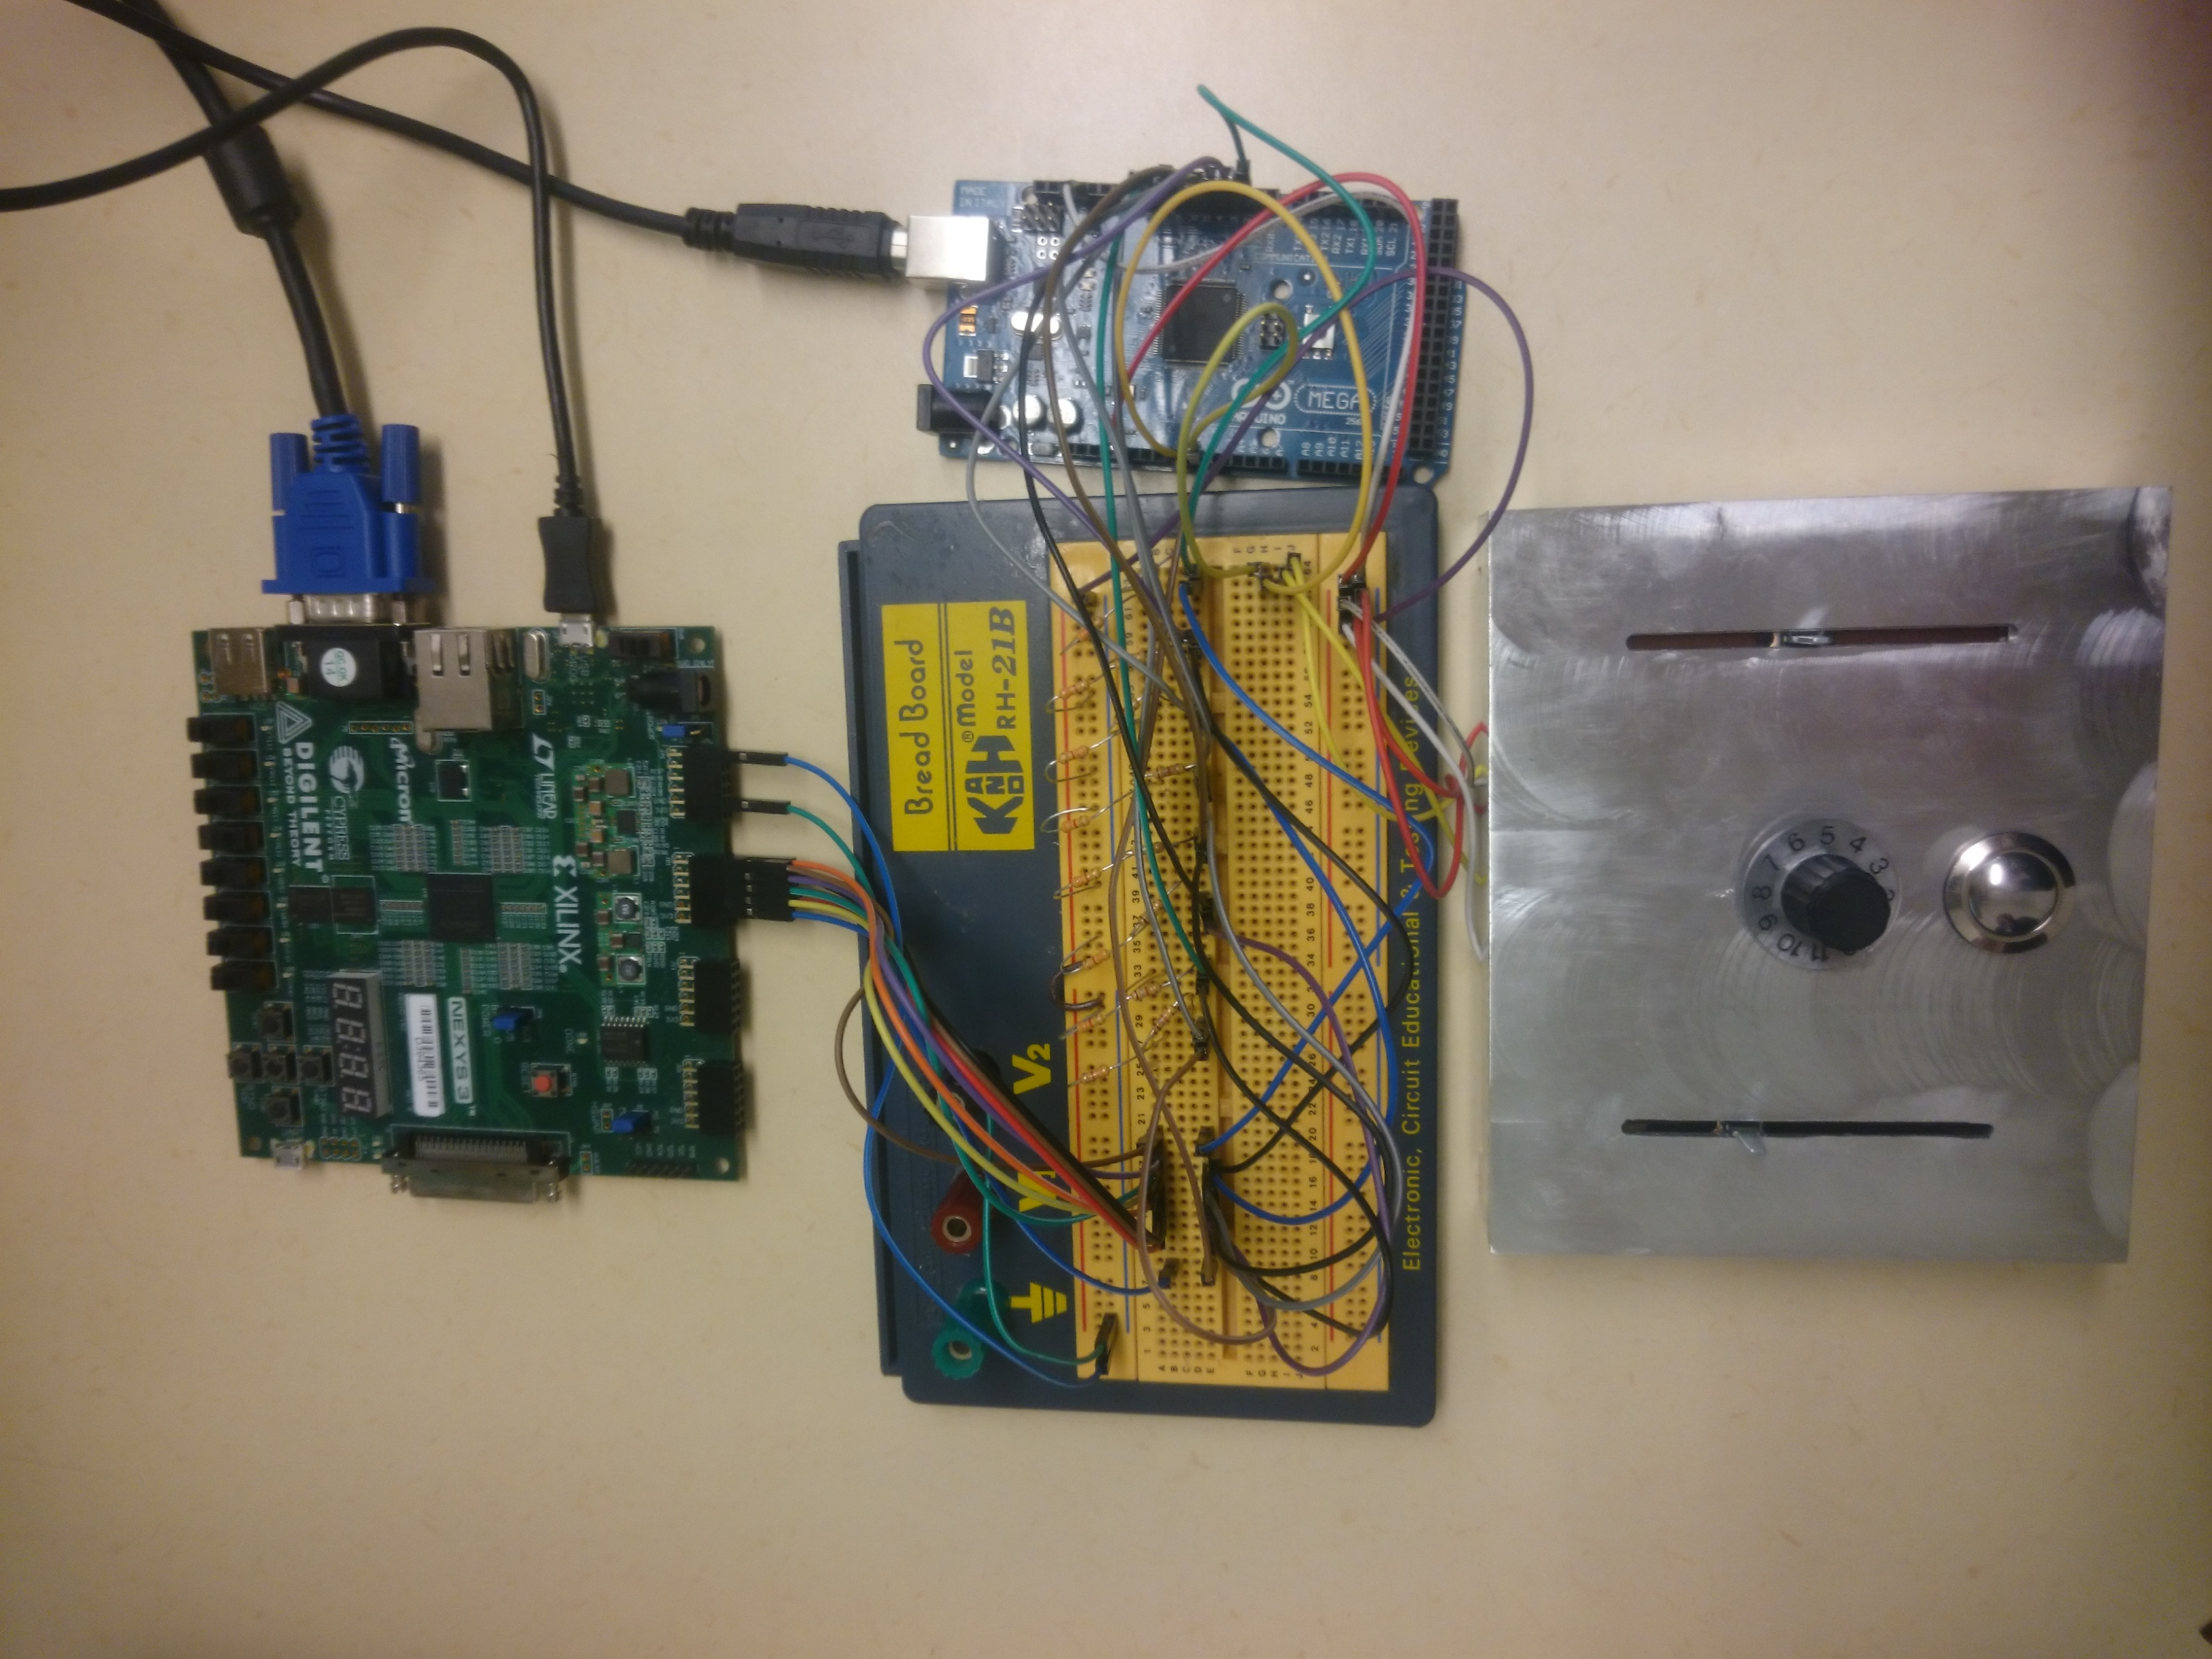
\includegraphics[scale=0.07]{../grafik/rapport-apparaten.JPG}
		\caption{Pong maskin}
		\label{fig:maskin}
	\end{figure}
\end{center}
\begin{center}
	\begin{figure}[H]
    	\centering
		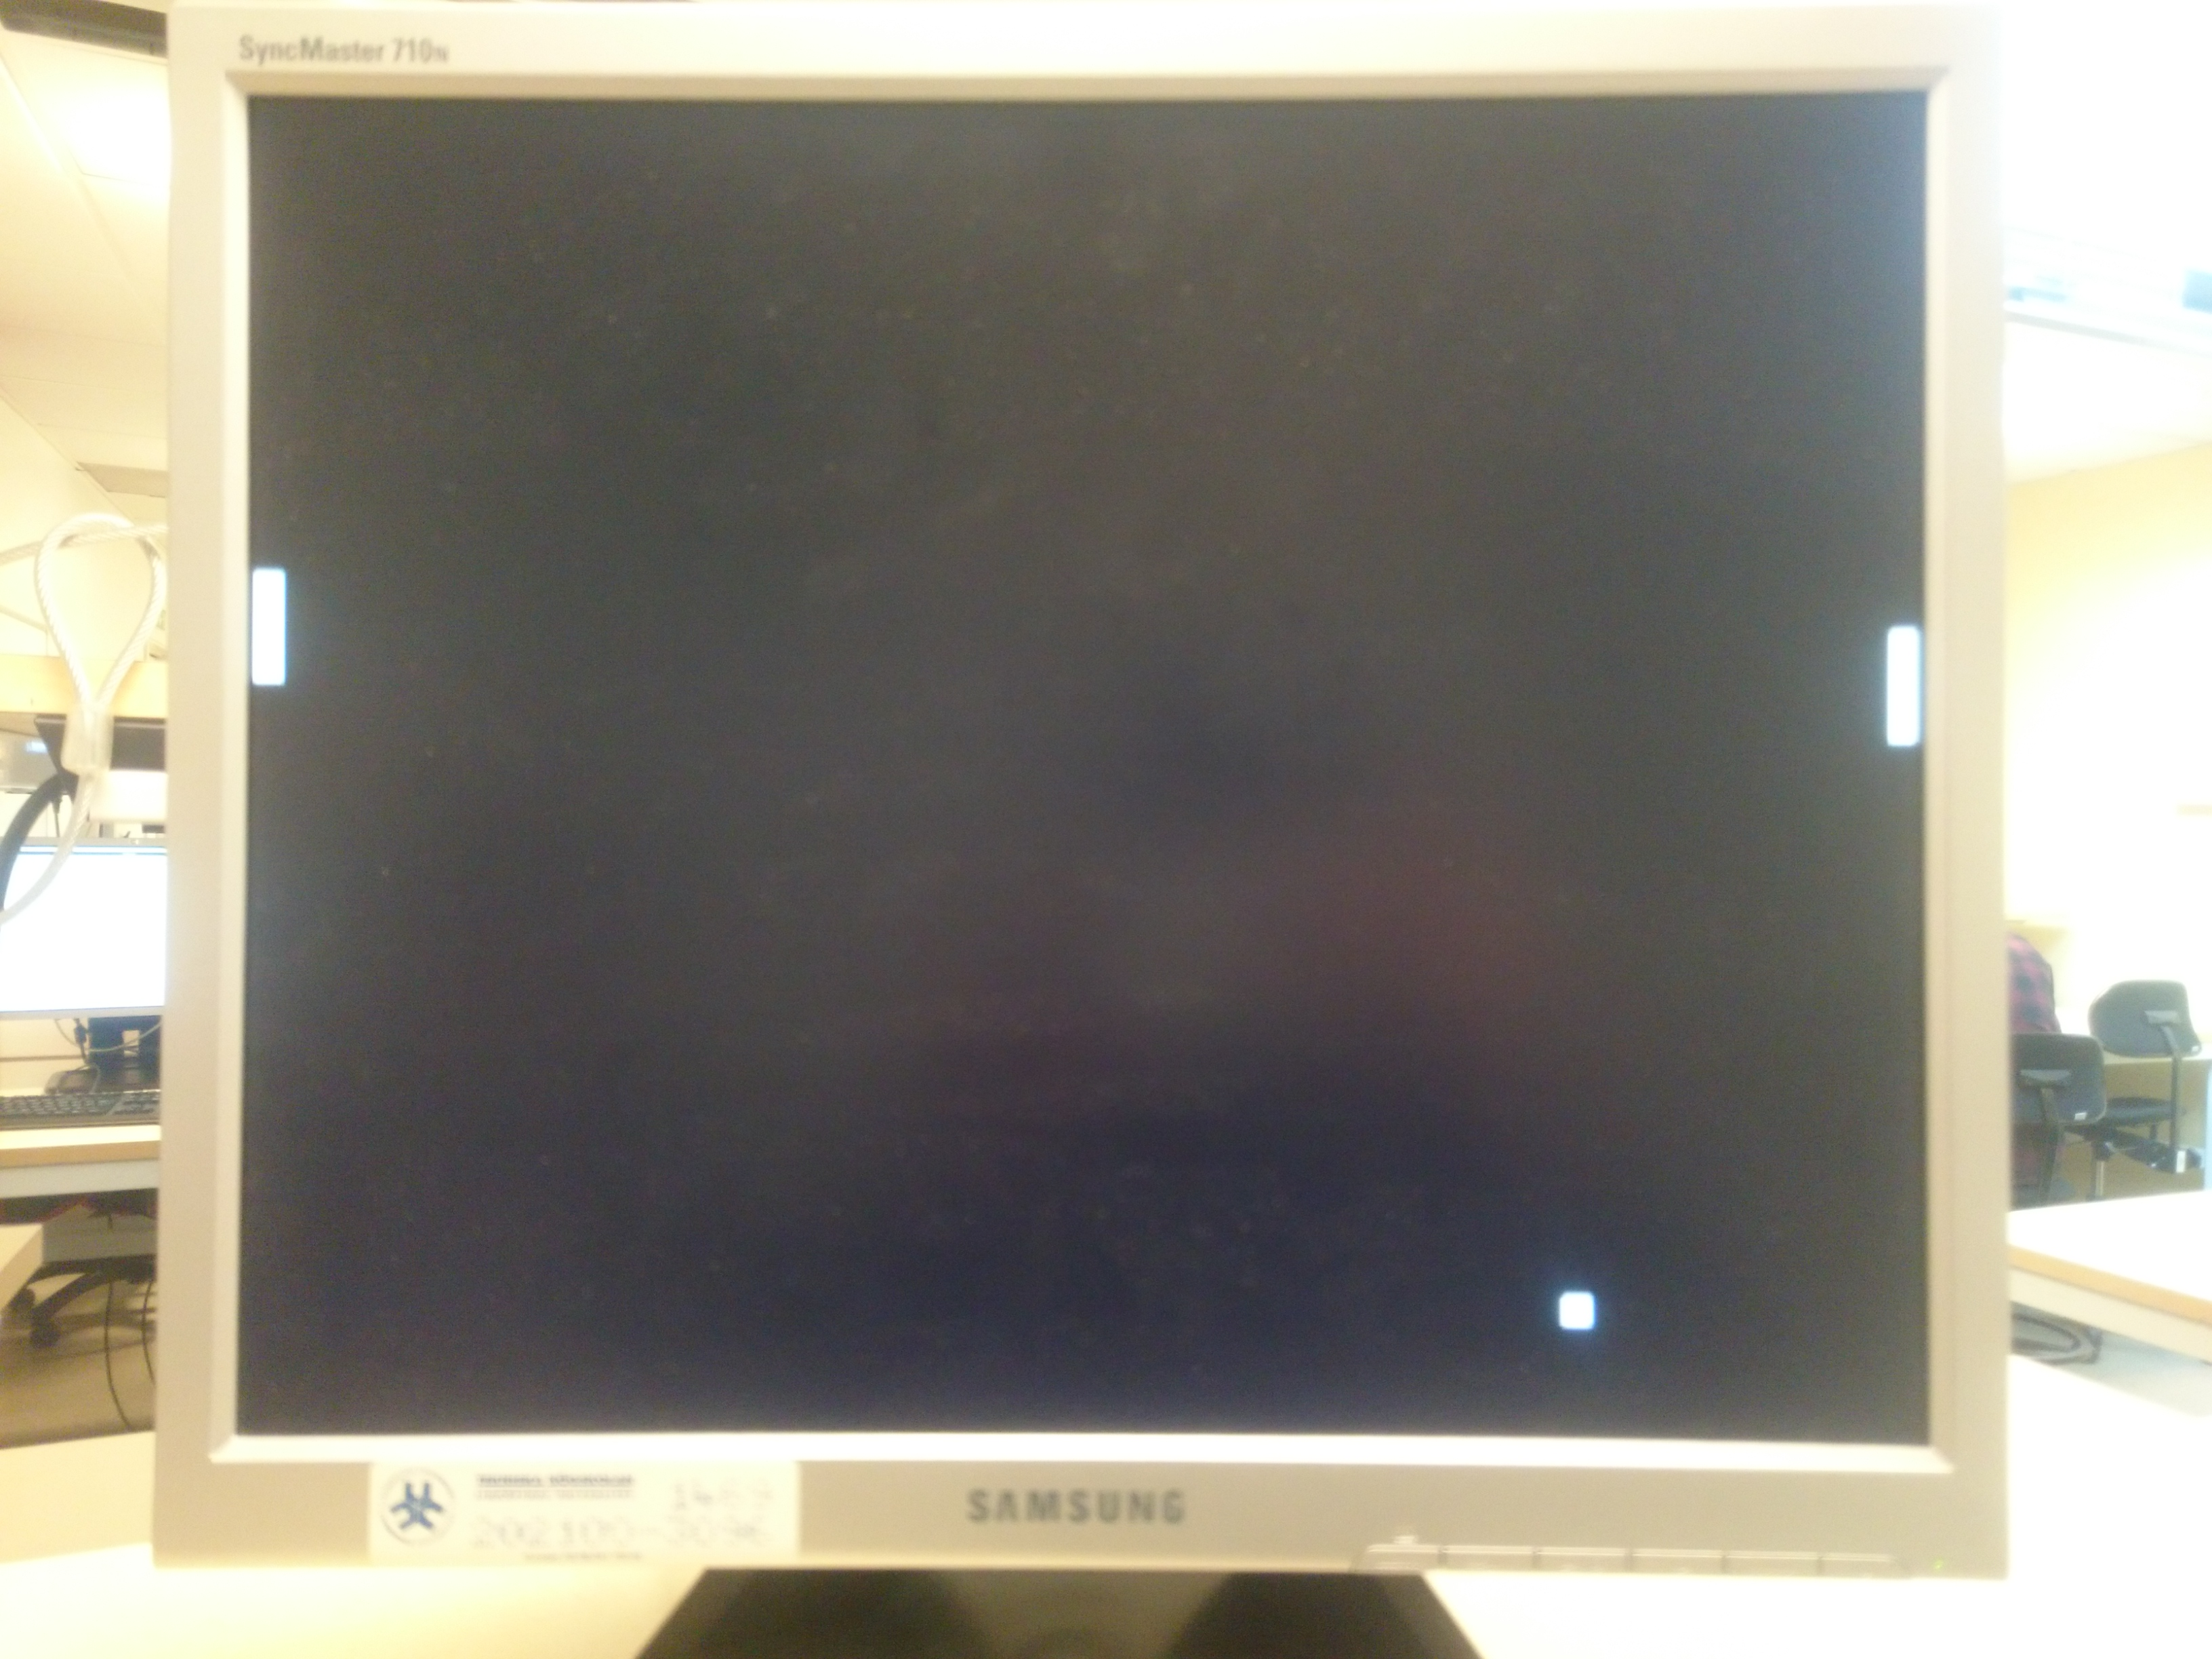
\includegraphics[scale=0.07]{../grafik/rapport-spel.JPG}
		\caption{VGA-Skärm}
		\label{fig:gui}
	\end{figure}
\end{center}

Två spelare använder varsin joystick som i sin tur styr spelarens stapel i spelet. Om någon av spelarna lyckas få bollen att passera motståndarens stapel får denna spelaren ett poäng som visas på toppen av skärmen. När en spelare fått tre poäng, vinner denna spelare och spelet startas om. Om man av någon anledning skulle vilja starta om innan en spelare fått tre poäng kan man använda en resetknapp, den svarta B8 knappen på Nexys-kortet.


\newpage

\iffalse
3. Teori
Här kan ett videoprojekt beskriva videoformatet, ett MIDI-projekt redogöra för MIDI-standarden ...
\fi


\section{Teori}
	Här gås teorietiska bakgrunderna för tekniken som använts i projektet.

\subsection{VGA}
	VGA (Video Graphics Array) introducerades först och främst på en IBM\circledR PS/2 dator i 1987 och en CRT-skärm. På Nexys 3 finns VGA, och därför användes detta till projektet. VGA standarden använder sig av en amplitudmodulerade rörliga elektroner för att visa en bild på monitorn. Standarden för visning och svepande av elektronstråle kräver en bra synkroniseringen. Detta för att den elektroniska kanonen som projicerar bilen måste hinna klart med alla rader innan bilden uppdateras. För att kanonen ska rikta om sig finns blankområdet, som ligger utanför det synliga fältet. Den tiden ger möjlighet för kanonen att ställa om sig till nästa rad. 
	Standarden har en feltolerans på $\pm0.5\%$, klockan i projektet skalas ner till så nära som möjligt för att kunna ge en hyfsad rätt frekvens \cite{vgasite}. I figur \ref{fig:vgateori} kan en god översikt ges av VGA-timingsen.


	\begin{center}
		\begin{figure}[H]
    		\centering
			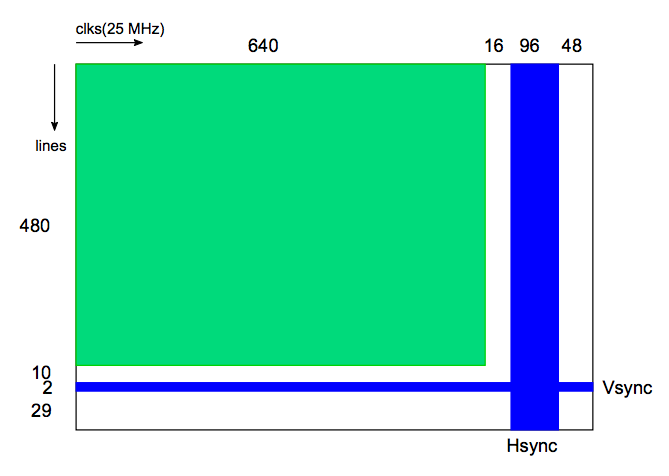
\includegraphics[scale=0.50]{../grafik/rapport-vgateori.png}
			\caption{VGA-timings \cite{vgapic}}
			\label{fig:vgateori}
		\end{figure}
	\end{center}


\subsection{Analog till digital konvertering}
	En analog till digital konvertering går ut på kvantisera de analoga signalerna exempelvis en elektrisk spänning till ett digitalt värde. Det analoga värdet kan anta vilka värden som helst, men det digitala enbart kan anta 0 eller 1. För att skapa en digital version behövs flera värden mätas och omvandlas. Vid en bestämd frekvens tas ett värde ut från den analoga signalen, detta kallas ett sampel. För att det inte ska bli någon interfereras läggs A/D-omvanldaren i ett \"sample-and-hold\" läge, och det utvalda värden kan därefter omvandlas. \cite{analogsite}.
	De fel man kan upptäcka på en A/D-omvandlare är ofta samma som felen som uppträder för en D/A-omvandlare. Vilka är:
	\begin{enumerate}
		\item Linjäritetsfel, kan ges upphov till av tillverkningstoleransen av motstånden.
		\item Offsetfel, balansen för nästkommande förstärkare är ur fas.
		\item Skalfel, en frekvens som inte är linjär.
	\end{enumerate}
	\cite{tsea82_2014}

	Här är ett exempel på hur en analog signals kurva ser ut, samt med alla sampel inritade.

	\begin{center}
		\begin{figure}[H]
    		\centering
			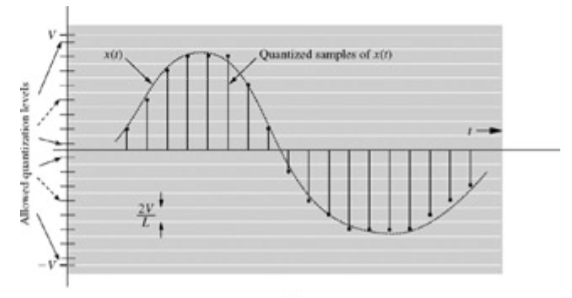
\includegraphics[scale=0.50]{../grafik/adc.png}
			\caption{VGA-timings \cite{adcpic}}
			\label{fig:adcteori}
		\end{figure}
	\end{center}
\newpage

\section{Hårdvara}
\subsection{Översikt}
	\begin{center}
		\begin{figure}[H]
    	\centering
			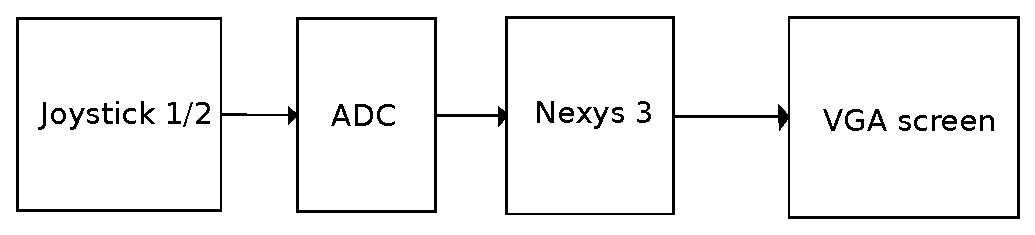
\includegraphics[scale=0.70]{../grafik/overview.eps}
			\caption{Översiktlig design}
			\label{fig:over}
		\end{figure}
	\end{center}
Joystickarna är insignaler till en A/D-omvandlare. Denna omvandlare är sedan i sin tur insignal till Nexys kortet där allt roligt händer. Kortet har en grafikmotor vars utsignal är insignal för en VGA bildskärm. 
\subsection{CPU}
	\begin{center}
		\begin{figure}[H]
    	\centering
			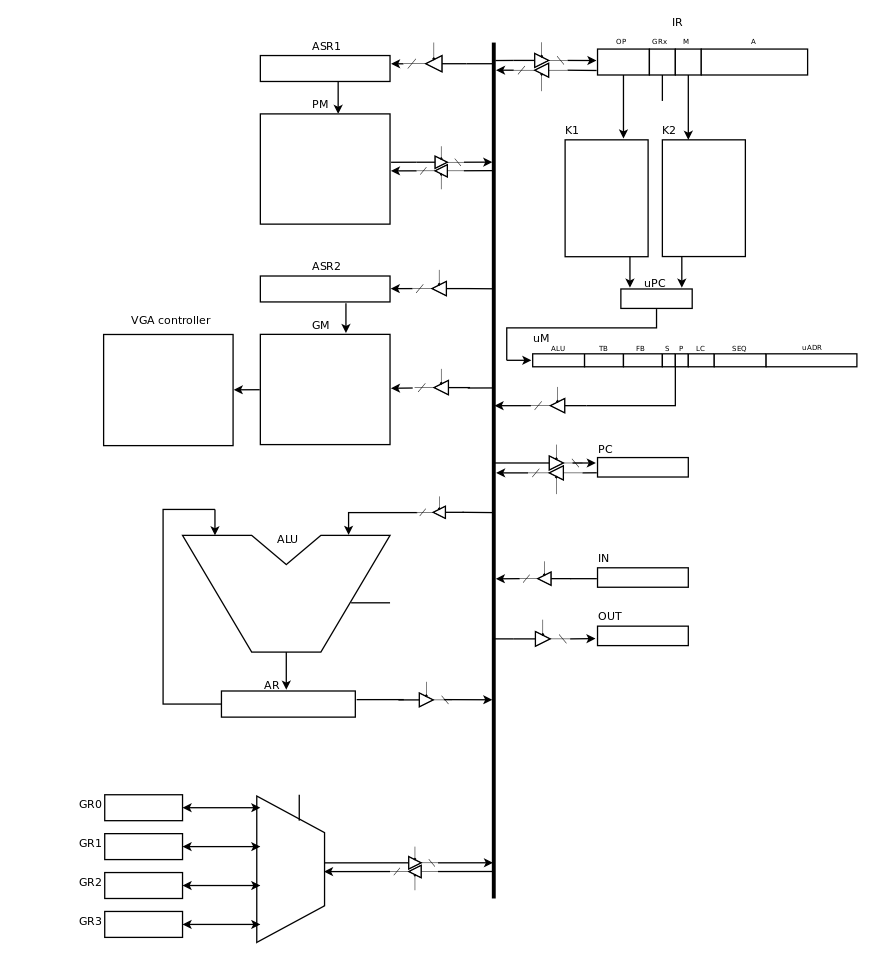
\includegraphics[scale=0.40]{../grafik/overall_design.png}
			\caption{CPU design}
			\label{fig:cpu}
		\end{figure}
	\end{center}
Ovan ses ett översiktligt blockschema på CPU:n. Denna är av Olle Roos modellen och är nästan identisk med CPU:n som användes i laboration 1. Det som lagts till är en grafikdel och en I/O enhet. Instruktionerna som används följer Olle Roos design, med ett par undantag: Instruktionen STOREV har lagts till för att kunna skriva till grafikminnet. Instruktionerna IN och OUT har lagts till för att hantera I/O enheten.
Både program och grafikminne implementerades som Block-RAM i Nexys-kortet. Dessa minnen är lika stora och består av 256 ord à 16 bitar.
\subsection{Grafik}
	\begin{center}
		\begin{figure}[H]
	    \centering
			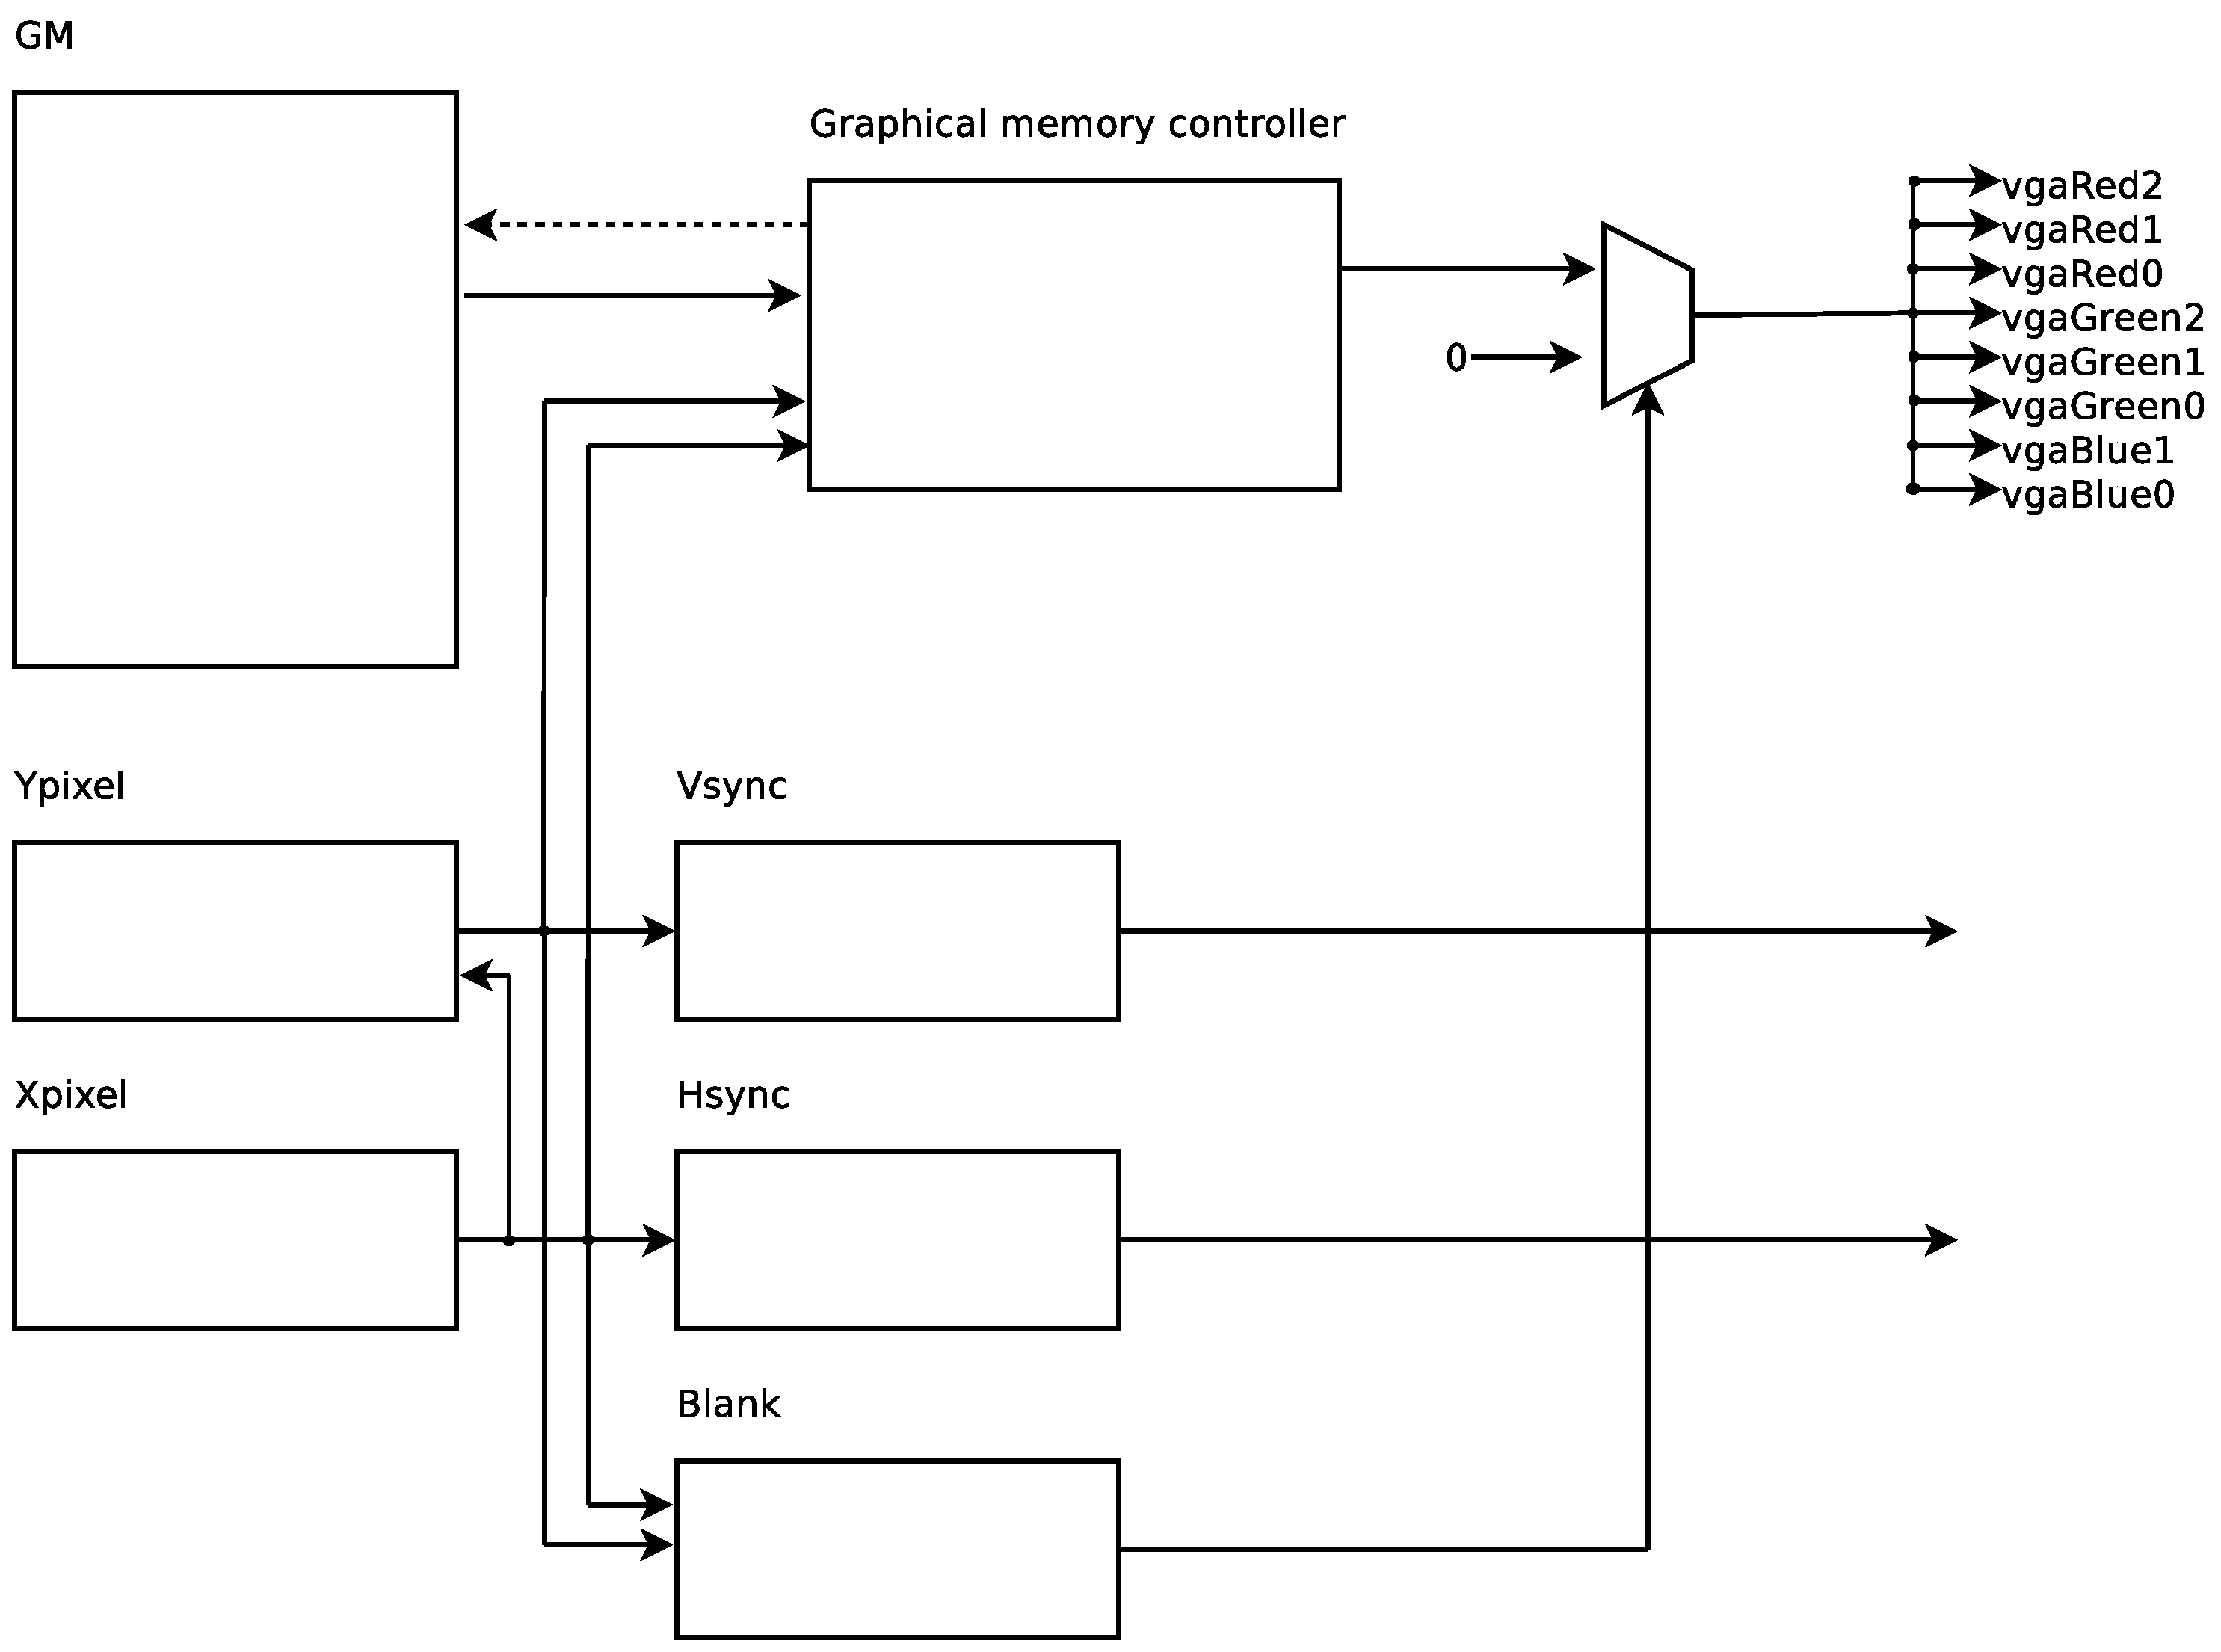
\includegraphics[scale=0.30]{../grafik/graphics.eps}
			\caption{VGA styrenhet}
			\label{fig:vga}
		\end{figure}
	\end{center}
Ovan ses ett översiktligt blockschema på VGA enheten. Enheten stödjer en upplösning på 640x480 pixlar och körs i 60Hz. Den stödjer två färger, svart och vit. Värderna som är valda medför att enheten måste ha en klocka på 25MHz. En spelpixel är definierad som 10x10 pixlar på VGA-skärmen, vilket resulterar i att den faktiska upplösningen är 64x48 pixlar. Grafikminnet är gjort så att en bit representerar en spelpixel. Det vill säga att fyra rader i minnet representerar en rad med spelpixlar på skärmen.
\subsection{I/O enheten}
	\begin{center}
		\begin{figure}[H]
    	\centering
			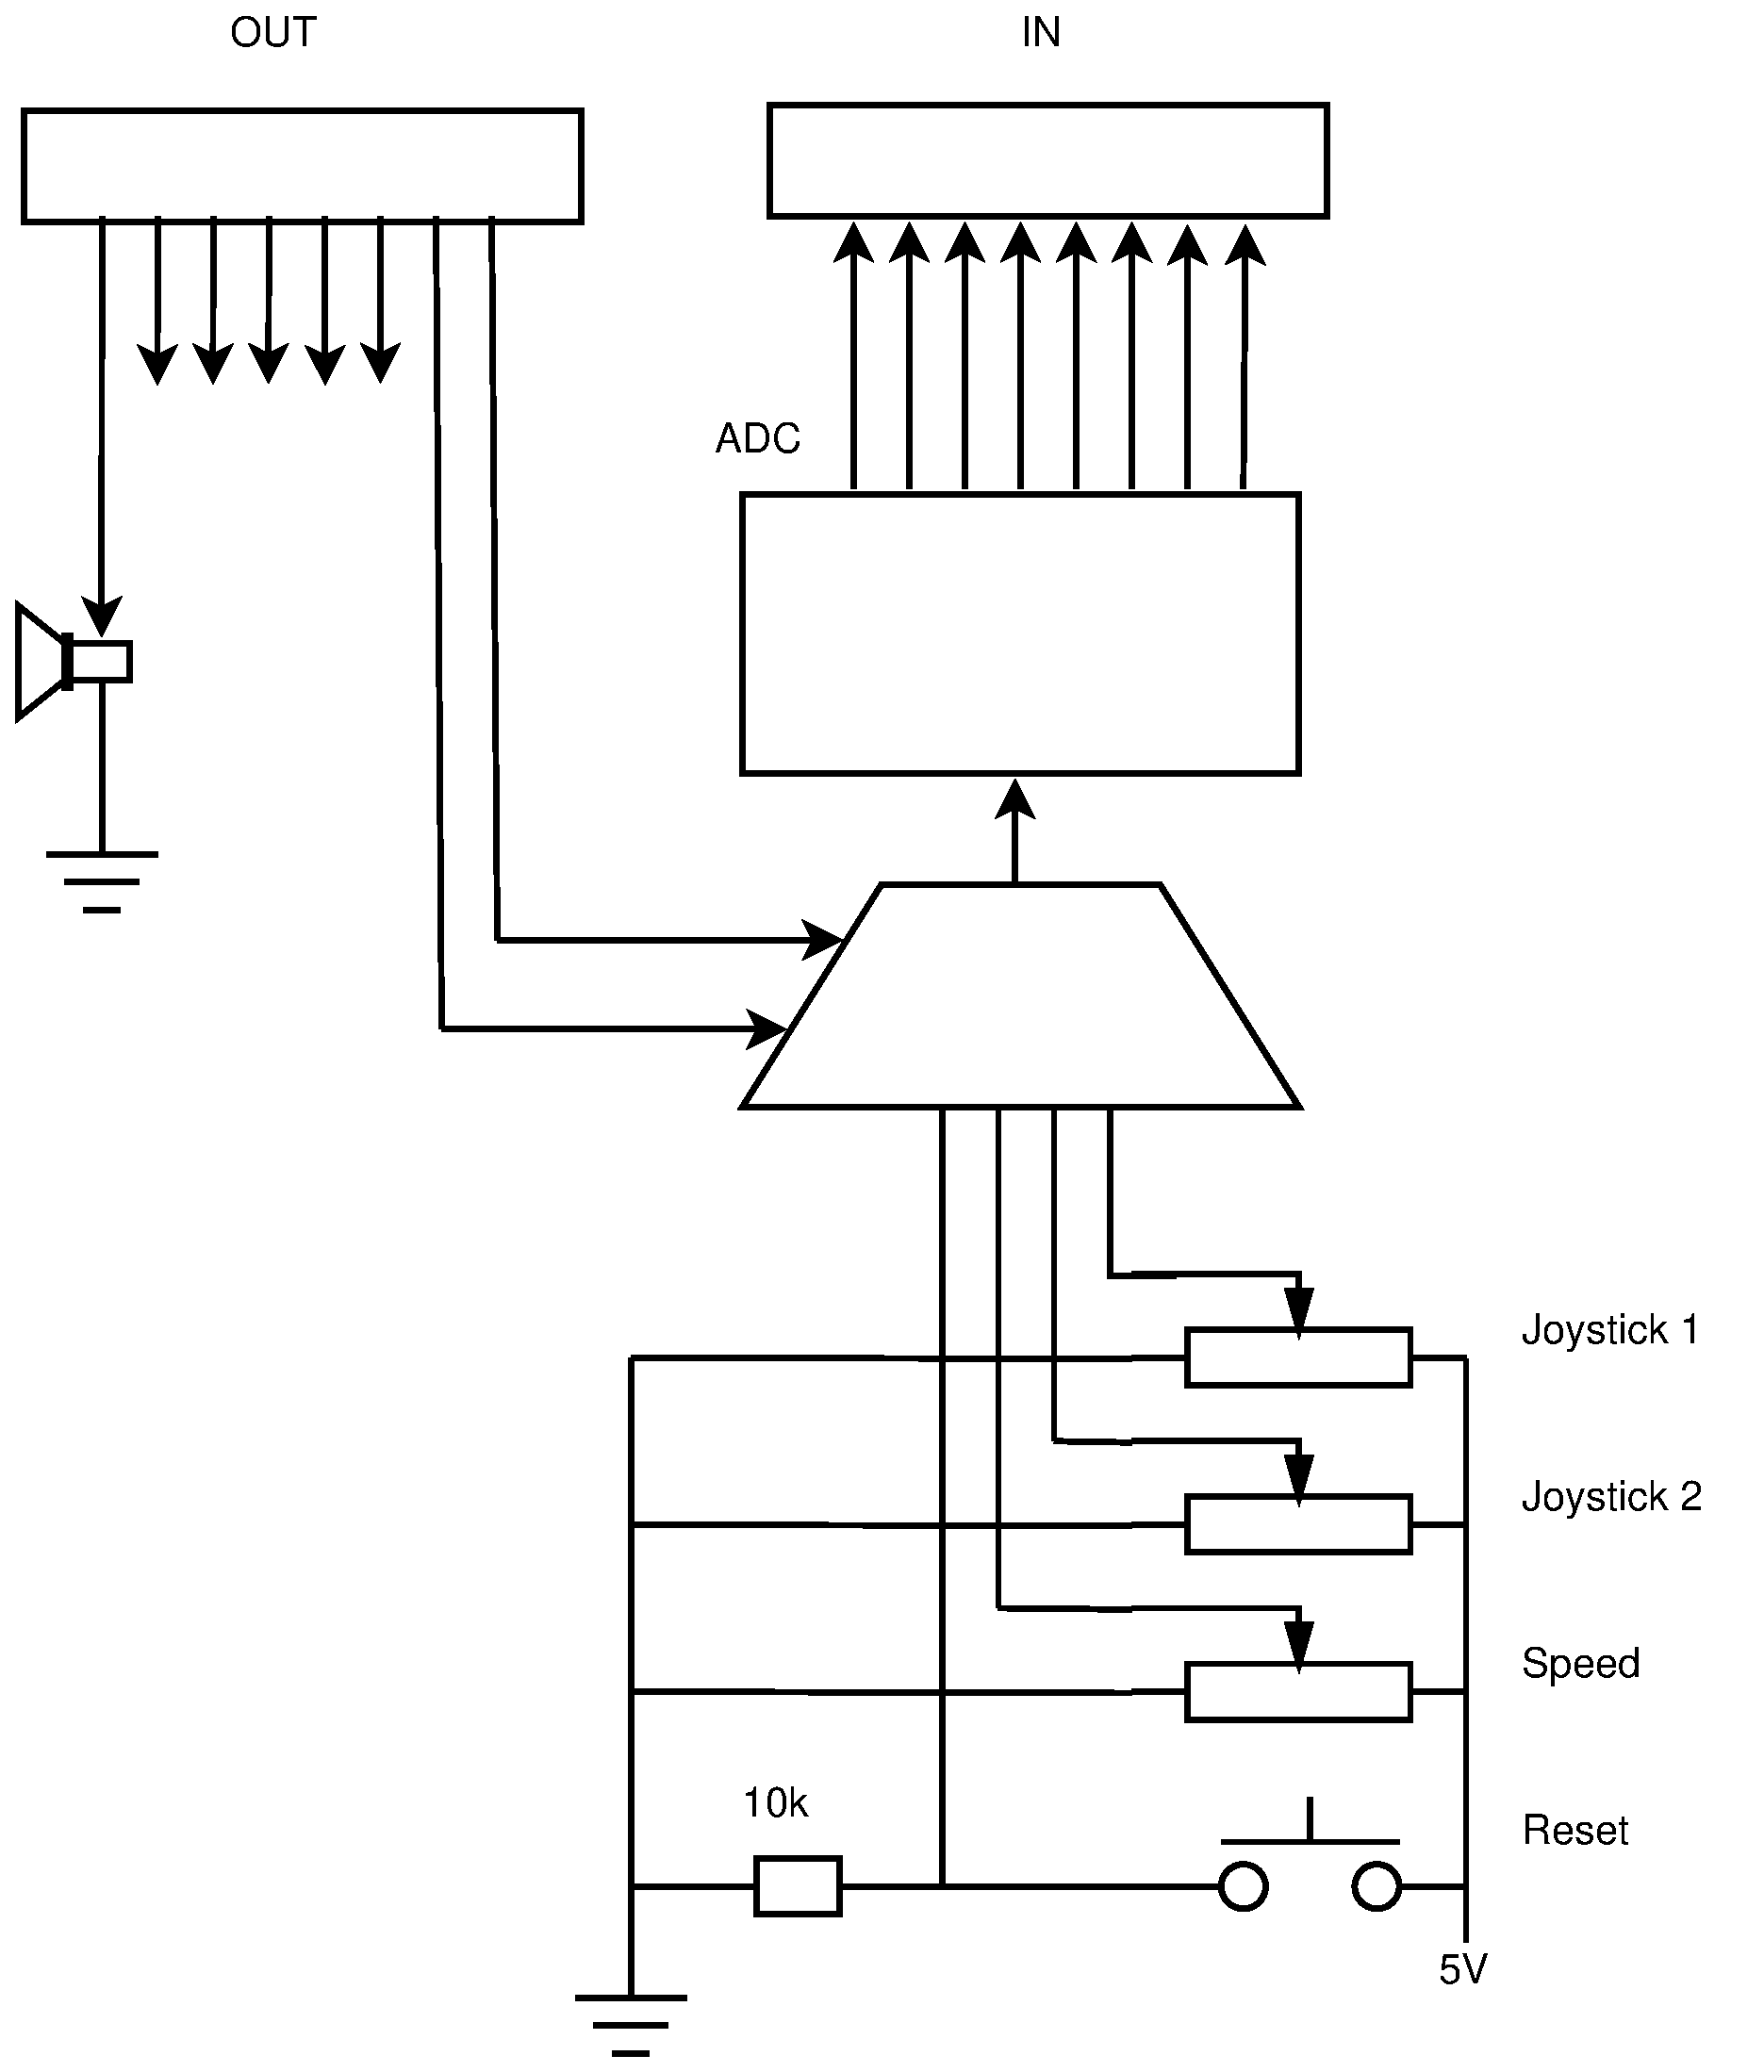
\includegraphics[scale=0.40]{../grafik/io.eps}
			\caption{IO design}
			\label{fig:joy}
		\end{figure}
	\end{center}
CPU:n har en 8 bitars ingång och en 8 bitars utgång som styrs av instruktionerna IN och OUT. Detta gör det möjligt att ha en extern AD-omvandlare och en analog mux för att kunna läsa av flera potentiometers. Dessa används för att styra staplarna i spelet.
Det är också möjligt att ha en extern reset knapp och hastighetskontroll. Dock är dessa funktioner inte implementerade.


\newpage

\section{Slutsatser}


Att välja analoga reglage till styrmedel tog kanske upp för mycket tid. Det var svårt att få dem att ansluta korrekt mellan varandra. Synkroniseringen mellan de analoga spakarna genom mux och avkodare vart nästintill omöjligt att få ett bra resultat ifrån. Eftersom det blev lite tidsbrist på slutet, ersattes den egna komponenten med en arduino som var länken från reglagen och fpga-kortet. Hade ett reglage med den exempelvis SPI använts hade de antagligen underlättat. Men gruppen valde analoga spakar och en egengjord modul för att det var mer av en rolig uppgift. Resultatet blev relativt spelvänligt, samt ett roligare projekt.
\\
Ett stort problem som gav många timmars felsökning var datorns problem med första blocket av grafikminnet. Lösningen blev att förskjuta allt med ett block, tyvärr fanns inte tid att felsöka vidare för att hitta den egentliga anledningen till problemet. 
\\
Lagringen för grafikminnet var genomtänkt från början men glömdes lite bort, då det inte var allt för aktuellt innan själva datorn fungerade. För att lösa detta hade vi en operand \'storev\', som fungerar utmärkt men blev troligtvis mer komplex än om åtanke hur de olika delarna av processorn skulle fylla samt avläsa grafikminnet gjorts tidigare. För att skriva till grafikminnet körs olika instruktioner som är uppdelade i x-position, y-position och färg. 
\\
Det som begränsade oss för att avklara bör-kraven, var storleken på data/programminnet. I nuläget används alla 256 rader, och det finns alltså ingen möjlighet att lägga in fler funktioner.

\newpage

\bibliography{referenser} 
\bibliographystyle{ieeetr}
\iffalse
\newpage

\iffalse
A. VHDL-kod
Inte själva VHDL-koden utan en förklaring av den. Det är ju inte säkert att VHDL-kodens processer och andra delar tydligt matchar dom blockchemor som ritats i hardvaruavsnittet. Då kan det vara lämpligt att förklara vad koden gör. Om VHDL-koden är väl strukturerad med bra kommentarer så räcker det gott att bara inkludera den i en tar-fil, enligt instruktioner ovan.
\fi
\newpage

\iffalse
B. Övriga listor
\fi

\fi

\end{document}
